%%%%% Set up %%%%%

% Set document style and font size
\documentclass[12pt]{article}\usepackage[]{graphicx}\usepackage[]{color}
%% maxwidth is the original width if it is less than linewidth
%% otherwise use linewidth (to make sure the graphics do not exceed the margin)
\makeatletter
\def\maxwidth{ %
  \ifdim\Gin@nat@width>\linewidth
    \linewidth
  \else
    \Gin@nat@width
  \fi
}
\makeatother

\definecolor{fgcolor}{rgb}{0.345, 0.345, 0.345}
\newcommand{\hlnum}[1]{\textcolor[rgb]{0.686,0.059,0.569}{#1}}%
\newcommand{\hlstr}[1]{\textcolor[rgb]{0.192,0.494,0.8}{#1}}%
\newcommand{\hlcom}[1]{\textcolor[rgb]{0.678,0.584,0.686}{\textit{#1}}}%
\newcommand{\hlopt}[1]{\textcolor[rgb]{0,0,0}{#1}}%
\newcommand{\hlstd}[1]{\textcolor[rgb]{0.345,0.345,0.345}{#1}}%
\newcommand{\hlkwa}[1]{\textcolor[rgb]{0.161,0.373,0.58}{\textbf{#1}}}%
\newcommand{\hlkwb}[1]{\textcolor[rgb]{0.69,0.353,0.396}{#1}}%
\newcommand{\hlkwc}[1]{\textcolor[rgb]{0.333,0.667,0.333}{#1}}%
\newcommand{\hlkwd}[1]{\textcolor[rgb]{0.737,0.353,0.396}{\textbf{#1}}}%
\let\hlipl\hlkwb

\usepackage{framed}
\makeatletter
\newenvironment{kframe}{%
 \def\at@end@of@kframe{}%
 \ifinner\ifhmode%
  \def\at@end@of@kframe{\end{minipage}}%
  \begin{minipage}{\columnwidth}%
 \fi\fi%
 \def\FrameCommand##1{\hskip\@totalleftmargin \hskip-\fboxsep
 \colorbox{shadecolor}{##1}\hskip-\fboxsep
     % There is no \\@totalrightmargin, so:
     \hskip-\linewidth \hskip-\@totalleftmargin \hskip\columnwidth}%
 \MakeFramed {\advance\hsize-\width
   \@totalleftmargin\z@ \linewidth\hsize
   \@setminipage}}%
 {\par\unskip\endMakeFramed%
 \at@end@of@kframe}
\makeatother

\definecolor{shadecolor}{rgb}{.97, .97, .97}
\definecolor{messagecolor}{rgb}{0, 0, 0}
\definecolor{warningcolor}{rgb}{1, 0, 1}
\definecolor{errorcolor}{rgb}{1, 0, 0}
\newenvironment{knitrout}{}{} % an empty environment to be redefined in TeX

\usepackage{alltt}

% File path to resources (style file etc)
\newcommand{\locRepo}{csas-style}

% Style file for DFO Technical Reports
\usepackage{\locRepo/tech-report}

% header-includes from R markdown entry


%%%%% Variables %%%%%

% New definitions: Title, year, report number, authors
% Protect lower case words (i.e., species names) in \Addlcwords{}, in "TechReport.sty"
\newcommand{\trTitle}{Title Here (\emph{Latin Species Name})}
\newcommand{\trYear}{20XX}
\newcommand{\trReportNum}{nnn}
% Optional
\newcommand{\trAuthFootA}{Email: \href{mailto:First.Author@dfo-mpo.gc.ca}{\nolinkurl{First.Author@dfo-mpo.gc.ca}} \textbar{} telephone: (250) 756-5555}
\newcommand{\trAuthsLong}{First. M. Last\textsuperscript{1} and Alex B. Smith\textsuperscript{2}}
\newcommand{\trAuthsBack}{Last, F.M. and Smith, A.B.}

% New definition: Address
\newcommand{\trAddy}{\textsuperscript{1}Pacific Biological Station\\
Fisheries and Oceans Canada, 3190 Hammond Bay Road\\
Nanaimo, British Columbia, V9T 6N7, Canada\\
\textsuperscript{2}Far, far away\\
Another Galaxy}

% Abstract
\newcommand{\trAbstract}{Here is the abstract text. Lorem ipsum dolor sit amet, consectetur adipisicing elit, sed do eiusmod tempor incididunt ut labore et dolore magna aliqua. Ut enim ad minim veniam, quis nostrud exercitation ullamco laboris nisi ut aliquip ex ea commodo consequat. Duis aute irure dolor in reprehenderit in voluptate velit esse cillum dolore eu fugiat nulla pariatur. Excepteur sint occaecat cupidatat non proident, sunt in culpa qui officia deserunt mollit anim id est laborum.}

% Resume (i.e., French abstract)
\newcommand{\trResume}{Voici le résumé. Lorem ipsum dolor sit amet, consectetur adipisicing elit, sed do eiusmod tempor incididunt ut labore et dolore magna aliqua. Ut enim ad minim veniam, quis nostrud exercitation ullamco laboris nisi ut aliquip ex ea commodo consequat. Duis aute irure dolor in reprehenderit in voluptate velit esse cillum dolore eu fugiat nulla pariatur. Excepteur sint occaecat cupidatat non proident, sunt in culpa qui officia deserunt mollit anim id est laborum.}

%%%%% Start %%%%%

% Start the document
\IfFileExists{upquote.sty}{\usepackage{upquote}}{}
\begin{document}

%%%% Front matter %%%%%

% Add the first few pages
\frontmatter

%%%%% Drafts %%%%%

%\linenumbers  % Line numbers
%\onehalfspacing  % Extra space between lines
\renewcommand{\headrulewidth}{0.5pt}  % Header line
\renewcommand{\footrulewidth}{0.5pt}  % footer line
%\pagestyle{fancy}\fancyhead[c]{Draft: Do not cite or circulate}  % Header text

%%%%% Main document %%%%%
\hypertarget{introduction}{%
\section{Introduction}\label{introduction}}

A reference (Edwards et al. \protect\hyperlink{ref-edwards2013}{2014}).
\begin{equation}
  1 + 1
  \label{eq:test}
\end{equation}
See Appendix~\ref{app:first-appendix}. See Equation \eqref{eq:test}.

\hypertarget{methods}{%
\section{Methods}\label{methods}}
\begin{figure}[htb]

{\centering \pdftooltip{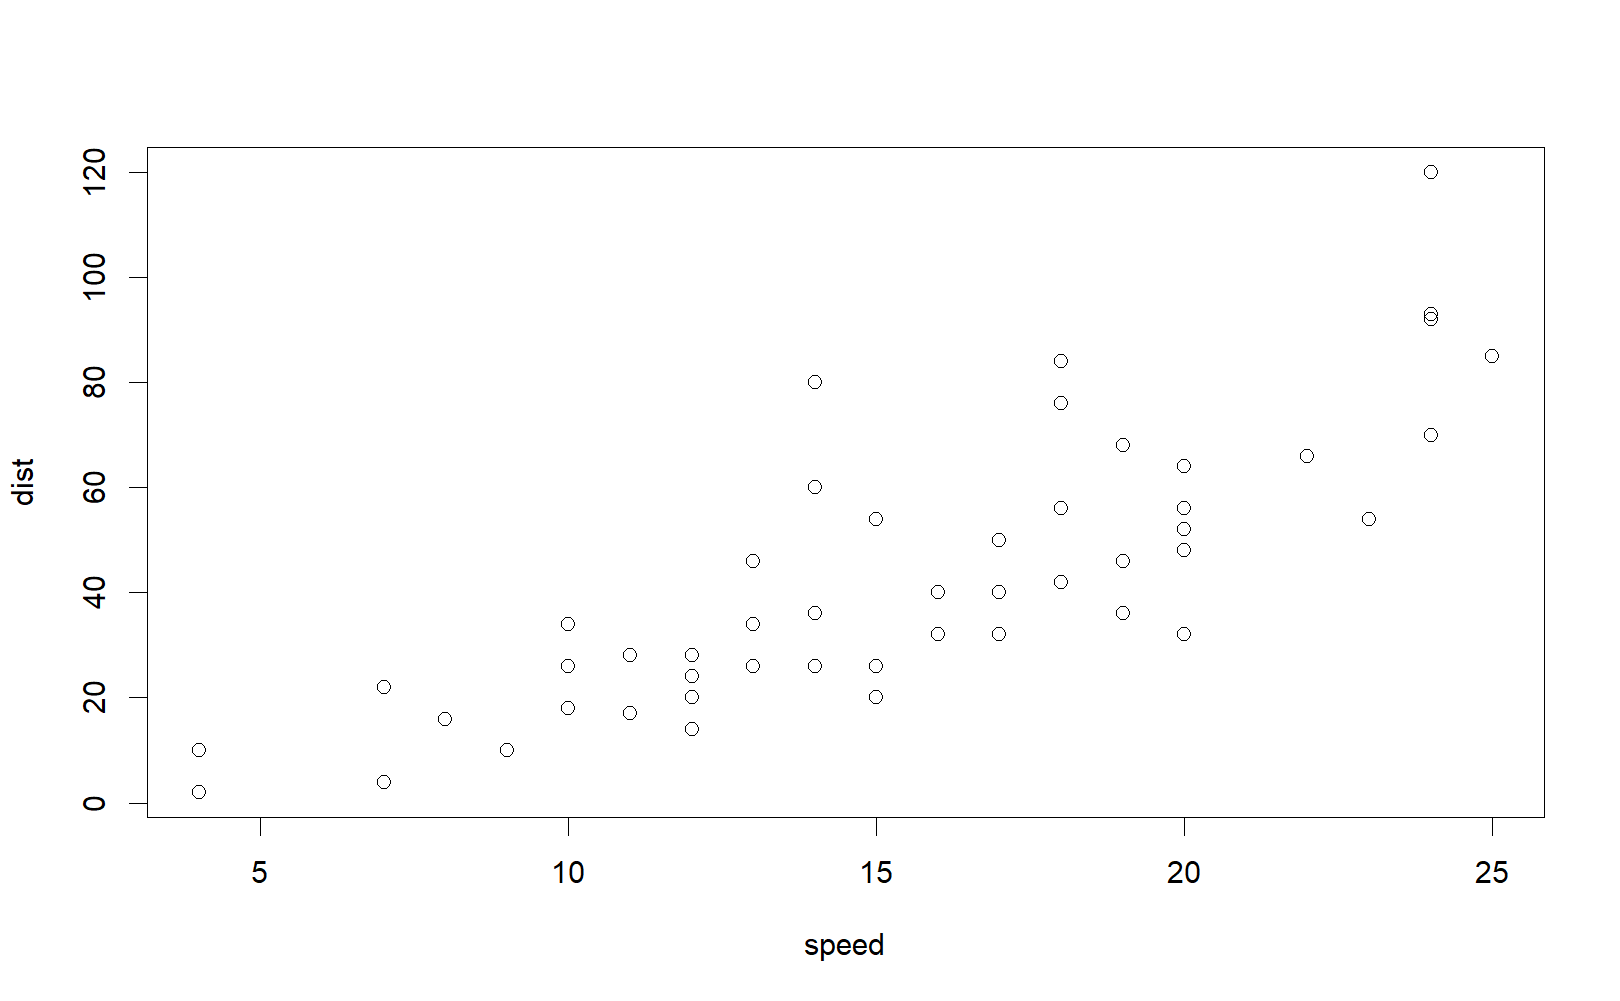
\includegraphics[width=6in]{knitr-figs-pdf/testfig-1}}{Figure \ref{fig:testfig}} 

}

\caption{Test figure with a caption will be numbered automatically.}\label{fig:testfig}
\end{figure}
\begin{longtable}[]{@{}crr@{}}
\caption{\label{tab:testtab}Test table with a caption will be numbered automatically.}\tabularnewline
\toprule
Year & Value 1 & Value 2\tabularnewline
\midrule
\endfirsthead
\toprule
Year & Value 1 & Value 2\tabularnewline
\midrule
\endhead
2018 & 1.12 & 31.9\tabularnewline
2019 & 2.32 & 2.8\tabularnewline
2020 & 3.67 & 112.2\tabularnewline
\bottomrule
\end{longtable}
See Table~\ref{tab:testtab} for the example table.

See Figure~\ref{fig:testfig} for the example figure.

\clearpage

\begingroup\fontsize{8}{10}\selectfont
\begin{landscape}
\begin{longtable}[t]{rrrrrrrrrrrrrrrr}
\caption{\label{tab:widelong}A long and wide table}\\
\toprule
\textbf{Year} & \textbf{1} & \textbf{2} & \textbf{3} & \textbf{4} & \textbf{5} & \textbf{6} & \textbf{7} & \textbf{8} & \textbf{9} & \textbf{10} & \textbf{11} & \textbf{12} & \textbf{13} & \textbf{14} & \textbf{15}\\
\midrule
\endfirsthead
\caption*{}\\
\toprule
\textbf{Year} & \textbf{1} & \textbf{2} & \textbf{3} & \textbf{4} & \textbf{5} & \textbf{6} & \textbf{7} & \textbf{8} & \textbf{9} & \textbf{10} & \textbf{11} & \textbf{12} & \textbf{13} & \textbf{14} & \textbf{15}\\
\midrule
\endhead
\
\endfoot
\bottomrule
\endlastfoot
1 & 19.2411 & 19.7738 & 21.2592 & 21.1894 & 20.0917 & 19.7906 & 19.8698 & 19.6201 & 19.5667 & 18.8685 & 20.9753 & 19.2946 & 18.5970 & 20.4236 & 20.9778\\
2 & 19.6336 & 22.0059 & 18.6117 & 20.0289 & 21.5583 & 20.8769 & 18.9169 & 17.9560 & 20.9047 & 18.6833 & 19.1835 & 21.0133 & 21.4141 & 19.5423 & 20.1842\\
3 & 20.6438 & 21.1024 & 19.3847 & 19.0995 & 21.2483 & 21.2573 & 18.6223 & 19.9137 & 19.5630 & 19.8847 & 20.4882 & 19.3153 & 20.8857 & 19.8459 & 18.3128\\
4 & 20.3422 & 18.3207 & 19.4930 & 19.5303 & 18.7291 & 20.4470 & 19.7965 & 19.4530 & 20.8002 & 21.3229 & 21.6977 & 18.7533 & 20.8929 & 19.9928 & 20.6933\\
5 & 19.1438 & 20.0784 & 18.8356 & 19.5221 & 19.5523 & 19.5587 & 19.8872 & 19.7473 & 19.5185 & 19.4818 & 19.8762 & 21.3841 & 19.9713 & 20.9304 & 21.4485\\
6 & 19.4510 & 21.1034 & 20.3820 & 19.8041 & 19.1509 & 19.6793 & 20.9998 & 21.8448 & 20.4162 & 19.0844 & 19.9335 & 19.4988 & 20.7282 & 19.1820 & 20.4392\\
7 & 21.2577 & 20.6907 & 19.1652 & 21.0687 & 19.9053 & 20.4375 & 21.5252 & 20.4191 & 18.1833 & 19.8759 & 18.9154 & 19.6810 & 20.1227 & 21.6056 & 20.2875\\
8 & 22.0201 & 22.0103 & 19.8903 & 19.8080 & 20.3176 & 19.8600 & 19.0183 & 20.9553 & 20.2709 & 21.7843 & 20.8344 & 19.1319 & 20.6285 & 20.6163 & 20.1397\\
9 & 19.0876 & 20.6929 & 18.9566 & 20.5390 & 19.8135 & 19.7088 & 21.1192 & 18.9203 & 20.8329 & 20.6739 & 20.8058 & 20.5577 & 20.5402 & 19.7161 & 19.6185\\
10 & 20.7346 & 19.8557 & 20.5005 & 18.9633 & 21.2204 & 19.7966 & 20.3159 & 21.9313 & 19.0685 & 18.8252 & 20.0464 & 18.7442 & 21.6269 & 17.8167 & 20.7009\\
11 & 21.7168 & 20.4739 & 20.3255 & 20.5712 & 20.2951 & 19.2707 & 20.7462 & 19.8577 & 20.8228 & 20.2162 & 19.6408 & 18.6414 & 19.4812 & 21.6867 & 20.0951\\
12 & 22.1024 & 18.8198 & 20.7193 & 21.2320 & 19.6121 & 19.0352 & 20.5734 & 17.7935 & 21.4362 & 19.5010 & 20.1630 & 20.4307 & 20.7729 & 19.4580 & 18.2815\\
13 & 20.1451 & 19.0575 & 18.8279 & 20.3475 & 21.0304 & 20.1268 & 20.5351 & 19.0998 & 19.0619 & 19.1783 & 19.9233 & 19.4108 & 19.5268 & 19.0673 & 21.2362\\
14 & 19.4382 & 21.8503 & 19.8969 & 19.2729 & 18.2582 & 19.0654 & 19.8559 & 18.9593 & 21.3603 & 18.5791 & 20.2398 & 21.4883 & 19.9981 & 20.1383 & 21.3056\\
15 & 19.6520 & 17.3880 & 20.4561 & 19.1539 & 19.1263 & 18.1802 & 21.3837 & 20.6784 & 19.6035 & 20.8466 & 20.4526 & 20.0545 & 20.3606 & 21.5054 & 19.6060\\
16 & 20.6150 & 18.9565 & 19.2460 & 18.5751 & 19.8619 & 20.7440 & 20.3730 & 20.7186 & 20.0045 & 19.0406 & 21.5337 & 20.6270 & 18.8708 & 19.0985 & 20.2972\\
17 & 18.9115 & 20.9106 & 19.1303 & 18.2507 & 21.9607 & 19.1801 & 20.7925 & 21.1910 & 20.8068 & 20.6120 & 20.5484 & 17.7993 & 20.7080 & 19.9829 & 21.3405\\
18 & 20.0360 & 19.6291 & 22.3263 & 20.5995 & 20.4818 & 21.1862 & 18.1693 & 20.9247 & 20.7630 & 20.0944 & 20.1493 & 18.9080 & 18.8689 & 19.2905 & 20.7034\\
19 & 20.7350 & 21.0607 & 20.1752 & 20.9509 & 20.0001 & 19.1853 & 20.8692 & 19.4151 & 20.2474 & 21.1021 & 21.1699 & 20.2067 & 20.6187 & 20.8222 & 19.0444\\
20 & 19.6475 & 21.6256 & 17.9667 & 21.4253 & 20.7134 & 19.8740 & 18.3126 & 21.4368 & 19.5692 & 19.2107 & 19.9930 & 20.9127 & 17.6544 & 18.4775 & 20.6722\\
21 & 19.0201 & 20.0676 & 18.7389 & 19.0651 & 18.6361 & 21.2034 & 21.9533 & 19.7004 & 19.3669 & 19.6819 & 17.6924 & 18.9530 & 20.1213 & 21.1436 & 21.2255\\
22 & 20.5616 & 20.4206 & 20.2637 & 18.5915 & 20.4497 & 18.4118 & 21.2158 & 18.9866 & 19.9175 & 20.9324 & 20.9570 & 20.1384 & 19.6171 & 19.2938 & 18.1722\\
23 & 20.3381 & 21.5573 & 20.1791 & 21.4675 & 21.3909 & 19.9367 & 21.6914 & 19.7973 & 20.1247 & 21.0616 & 19.9264 & 19.2872 & 20.9286 & 19.1099 & 21.9643\\
24 & 19.9839 & 19.9261 & 20.1247 & 20.2634 & 20.0499 & 21.3152 & 20.4761 & 20.5678 & 20.2420 & 20.3552 & 20.5225 & 20.4556 & 21.0524 & 19.3445 & 21.2300\\
25 & 20.7106 & 19.0059 & 20.2222 & 20.7918 & 21.3896 & 18.5473 & 19.1485 & 21.5133 & 19.4891 & 20.4834 & 19.3537 & 19.5952 & 21.2437 & 19.4098 & 19.5874\\
26 & 19.7459 & 20.3352 & 21.2377 & 19.2054 & 19.2168 & 19.3475 & 20.8863 & 20.1369 & 19.4189 & 19.3275 & 21.0792 & 20.6021 & 17.5844 & 20.2198 & 19.8647\\
27 & 20.5619 & 18.8323 & 20.6503 & 19.4309 & 19.3726 & 18.8271 & 20.3582 & 19.9612 & 21.0377 & 18.9133 & 21.1046 & 19.6337 & 20.8028 & 20.3938 & 18.5375\\
28 & 18.9419 & 21.1568 & 20.4857 & 20.4641 & 20.0189 & 21.0298 & 19.9432 & 19.7567 & 18.2576 & 19.4969 & 17.7737 & 19.6974 & 19.7649 & 20.7120 & 20.3097\\
29 & 21.9994 & 19.3674 & 19.4314 & 19.9976 & 18.8898 & 19.3314 & 22.0228 & 19.6992 & 19.8148 & 19.9987 & 19.4850 & 18.7954 & 21.4278 & 20.9648 & 18.0207\\
30 & 22.6265 & 19.5802 & 20.0636 & 21.3527 & 18.9154 & 19.7709 & 19.3678 & 19.2657 & 19.5570 & 19.1958 & 18.8146 & 17.6969 & 18.4731 & 20.9820 & 19.6783\\
31 & 20.8549 & 18.9879 & 19.4568 & 19.1520 & 20.3002 & 20.6782 & 19.6637 & 20.2064 & 20.7801 & 19.5869 & 20.1707 & 21.5068 & 20.4495 & 21.3375 & 19.6617\\
32 & 20.9155 & 22.0771 & 18.9730 & 18.9010 & 19.0293 & 19.9286 & 21.0553 & 21.0580 & 21.2024 & 19.7231 & 19.3103 & 20.3642 & 21.0833 & 21.4901 & 22.8511\\
33 & 21.3165 & 20.7315 & 18.2365 & 18.1825 & 20.6080 & 17.7713 & 21.8521 & 19.8419 & 19.8392 & 20.6486 & 20.9242 & 19.1342 & 20.1715 & 20.5416 & 19.2449\\
34 & 20.4602 & 19.8502 & 21.1365 & 20.1353 & 20.5454 & 19.6969 & 20.2234 & 19.5989 & 21.2743 & 20.4182 & 19.2935 & 19.0047 & 20.2728 & 19.5383 & 20.4616\\
35 & 20.5412 & 19.6186 & 20.0687 & 18.8519 & 19.8323 & 20.6968 & 20.0618 & 20.2261 & 18.9834 & 19.3343 & 20.1480 & 19.9111 & 19.9300 & 19.5182 & 20.5020\\
36 & 19.5620 & 21.6738 & 19.3826 & 21.5949 & 20.9367 & 19.9174 & 20.4844 & 21.0906 & 22.4904 & 17.3770 & 16.9184 & 19.9152 & 21.6918 & 20.6214 & 21.1922\\
37 & 19.3318 & 21.7798 & 18.2788 & 20.6436 & 19.4774 & 20.0515 & 20.2189 & 20.5109 & 20.7346 & 21.0422 & 21.3500 & 19.8967 & 19.7979 & 18.2892 & 21.3503\\
38 & 21.1388 & 20.0553 & 20.2366 & 18.2813 & 19.8511 & 18.3272 & 20.8381 & 21.2369 & 19.8362 & 19.6313 & 19.2804 & 20.2440 & 21.5028 & 19.0873 & 18.6955\\
39 & 21.0902 & 19.0104 & 19.3621 & 18.7025 & 21.6964 & 18.5540 & 20.2623 & 20.6896 & 19.6960 & 18.4772 & 21.1876 & 20.2518 & 20.9155 & 20.4077 & 20.3954\\
40 & 18.8729 & 21.1914 & 20.0561 & 19.6752 & 20.0180 & 19.6935 & 19.1891 & 18.9639 & 20.2142 & 18.5148 & 19.5906 & 19.5788 & 21.4074 & 19.7591 & 19.5917\\
41 & 18.4372 & 19.2259 & 19.8868 & 18.5422 & 20.8862 & 18.2569 & 20.6400 & 19.8518 & 19.3096 & 19.9960 & 18.7270 & 20.0105 & 19.4223 & 18.6479 & 19.5412\\
42 & 22.3390 & 20.4911 & 20.5466 & 18.2894 & 20.0819 & 20.2699 & 20.6724 & 20.2818 & 20.4649 & 17.3310 & 20.0087 & 20.8272 & 18.8810 & 19.1942 & 19.1019\\
43 & 18.3894 & 18.3366 & 21.0536 & 18.8476 & 19.2586 & 19.3841 & 19.7773 & 21.0981 & 18.8810 & 21.0094 & 19.6561 & 18.8319 & 18.5557 & 19.2002 & 19.9210\\
44 & 21.7821 & 19.6856 & 21.3925 & 18.6361 & 19.5304 & 18.1611 & 21.2999 & 19.7631 & 20.1651 & 18.9917 & 21.5040 & 20.7177 & 19.0651 & 19.0807 & 19.4058\\
45 & 19.9701 & 19.2322 & 19.8448 & 20.7732 & 20.6471 & 20.9745 & 19.9093 & 20.4542 & 19.4419 & 19.9672 & 20.4945 & 20.1733 & 21.3960 & 21.6325 & 19.0464\\*
\end{longtable}
\end{landscape}
\endgroup{}

\clearpage

\hypertarget{results}{%
\section{Results}\label{results}}

\begingroup\fontsize{8}{10}\selectfont
\begin{landscape}
\begin{longtable}[t]{>{\raggedright\arraybackslash}p{3.6 cm}rrrrrrrrrrrrrr}
\caption{\label{tab:unnamed-chunk-1}Example catch table}\\
\toprule
\multicolumn{1}{c}{Tows} & \multicolumn{1}{c}{1} & \multicolumn{1}{c}{2} & \multicolumn{1}{c}{3} & \multicolumn{1}{c}{4} & \multicolumn{1}{c}{5} & \multicolumn{1}{c}{6} & \multicolumn{1}{c}{7} & \multicolumn{1}{c}{8} & \multicolumn{1}{c}{9} & \multicolumn{1}{c}{10} & \multicolumn{1}{c}{11} & \multicolumn{1}{c}{12} & \multicolumn{1}{c}{13} & \multicolumn{1}{c}{14} \\
\cmidrule(l{3pt}r{3pt}){1-1} \cmidrule(l{3pt}r{3pt}){2-2} \cmidrule(l{3pt}r{3pt}){3-3} \cmidrule(l{3pt}r{3pt}){4-4} \cmidrule(l{3pt}r{3pt}){5-5} \cmidrule(l{3pt}r{3pt}){6-6} \cmidrule(l{3pt}r{3pt}){7-7} \cmidrule(l{3pt}r{3pt}){8-8} \cmidrule(l{3pt}r{3pt}){9-9} \cmidrule(l{3pt}r{3pt}){10-10} \cmidrule(l{3pt}r{3pt}){11-11} \cmidrule(l{3pt}r{3pt}){12-12} \cmidrule(l{3pt}r{3pt}){13-13} \cmidrule(l{3pt}r{3pt}){14-14} \cmidrule(l{3pt}r{3pt}){15-15}
\textbf{Event.Number} & \textbf{X19} & \textbf{X22} & \textbf{X23} & \textbf{X26} & \textbf{X27} & \textbf{X28} & \textbf{X29} & \textbf{X30} & \textbf{X33} & \textbf{X36} & \textbf{X37} & \textbf{X38} & \textbf{X39} & \textbf{X42}\\
\midrule
\endfirsthead
\caption*{}\\
\toprule
\textbf{Event.Number} & \textbf{X19} & \textbf{X22} & \textbf{X23} & \textbf{X26} & \textbf{X27} & \textbf{X28} & \textbf{X29} & \textbf{X30} & \textbf{X33} & \textbf{X36} & \textbf{X37} & \textbf{X38} & \textbf{X39} & \textbf{X42}\\
\midrule
\endhead
\
\endfoot
\bottomrule
\endlastfoot
AMERICAN SHAD & NA & NA & NA & NA & NA & NA & NA & NA & NA & NA & NA & NA & NA & NA\\
ARROWTOOTH FLOUNDER, TURBOT & NA & NA & NA & NA & NA & 0.04 & NA & NA & NA & NA & NA & NA & NA & NA\\
BLACK ROCKFISH & 0.25 & NA & 0.10 & NA & NA & NA & NA & NA & NA & NA & NA & NA & NA & NA\\
BLUE SHARK & NA & NA & NA & NA & NA & NA & NA & NA & NA & NA & NA & NA & NA & NA\\
BOREAL CLUBHOOK SQUID & NA & NA & NA & NA & NA & NA & NA & NA & NA & NA & NA & NA & NA & NA\\
CALIFORNIA SEA LION & NA & NA & NA & NA & NA & NA & NA & NA & NA & NA & NA & NA & NA & NA\\
CALYCOPSIS & NA & NA & NA & NA & NA & NA & NA & NA & NA & NA & NA & NA & NA & NA\\
CANARY ROCKFISH & NA & NA & NA & NA & NA & NA & NA & NA & NA & NA & NA & NA & NA & NA\\
CHINOOK SALMON & 2.27 & NA & 6.99 & NA & 0.41 & NA & NA & 0.69 & 5.41 & NA & NA & 11.09 & NA & NA\\
CHUM SALMON & NA & NA & 9.17 & NA & 0.03 & NA & 6.33 & NA & NA & NA & NA & 0.07 & 0.95 & NA\\
CODFISHES & NA & NA & NA & NA & NA & NA & NA & NA & NA & NA & NA & NA & NA & NA\\
COHO SALMON & NA & NA & 0.06 & NA & 2.36 & NA & 0.03 & NA & NA & NA & NA & NA & NA & NA\\
COMB JELLYFISH & NA & NA & NA & NA & NA & NA & NA & NA & NA & NA & NA & NA & NA & NA\\
COPPER ROCKFISH & NA & NA & NA & NA & NA & NA & NA & NA & NA & NA & NA & NA & NA & NA\\
DARKBLOTCHED ROCKFISH & NA & NA & NA & NA & NA & NA & NA & NA & NA & NA & NA & NA & NA & NA\\
DINNER PLATE JELLYFISH & NA & NA & NA & NA & NA & NA & NA & NA & 1.88 & 0.58 & NA & NA & NA & NA\\
EULACHON & NA & NA & NA & 0.12 & NA & 0.06 & NA & NA & NA & NA & NA & NA & NA & NA\\
EUPHAUSIIDS & NA & NA & NA & NA & NA & 1.24 & NA & NA & NA & 5.03 & NA & NA & NA & NA\\
FLATFISHES & NA & NA & NA & NA & NA & 0.08 & NA & NA & NA & NA & NA & NA & NA & NA\\
FRIED EGG JELLY & NA & NA & NA & 2.20 & NA & NA & NA & NA & NA & NA & NA & NA & NA & 0.05\\
GREENLINGS & NA & NA & NA & NA & NA & NA & NA & NA & NA & NA & NA & NA & NA & NA\\
GREENSTRIPED ROCKFISH & NA & NA & NA & NA & NA & NA & NA & NA & NA & NA & NA & NA & NA & NA\\
ISOPODS & NA & NA & NA & NA & NA & NA & NA & NA & NA & NA & NA & NA & NA & NA\\
JACK MACKEREL & NA & NA & NA & NA & NA & NA & NA & NA & NA & NA & NA & NA & NA & NA\\
JELLYFISH & NA & NA & NA & NA & NA & NA & NA & NA & NA & 4.02 & 2.34 & NA & 11.53 & 2.56\\
LANTERNFISH & NA & NA & NA & NA & NA & NA & NA & NA & NA & NA & NA & NA & NA & NA\\
LIONS MANE & NA & NA & NA & NA & NA & NA & NA & NA & NA & 4.29 & NA & NA & 7.43 & 6.80\\
LUMPFISHES AND SNAILFISHES & NA & NA & NA & NA & NA & NA & NA & NA & NA & NA & NA & NA & NA & NA\\
MOON JELLYFISH & NA & NA & NA & NA & NA & NA & 0.47 & NA & NA & NA & NA & NA & NA & 0.36\\
NORTH PACIFIC SPINY DOGFISH & NA & NA & NA & NA & NA & NA & NA & NA & NA & NA & NA & NA & NA & NA\\
NORTHERN ANCHOVY & NA & NA & NA & NA & 0.05 & NA & NA & NA & NA & NA & NA & NA & NA & NA\\
NORTHERN SPEARNOSE POACHER & NA & NA & NA & NA & NA & NA & NA & NA & NA & NA & NA & NA & NA & NA\\
OCEAN SUNFISH & NA & NA & NA & NA & NA & NA & NA & NA & NA & NA & NA & NA & NA & NA\\
OPALESCENT INSHORE SQUID & 0.14 & NA & NA & NA & 1.70 & NA & 0.12 & NA & NA & NA & NA & 0.08 & NA & NA\\
PACIFIC HAKE & NA & NA & NA & NA & NA & NA & NA & NA & NA & NA & NA & NA & NA & NA\\
PACIFIC HERRING & 5.32 & NA & 0.50 & 826.75 & 84.18 & 3.62 & 11.23 & NA & NA & NA & 1.26 & 23.78 & NA & NA\\
PACIFIC LAMPREY & NA & NA & NA & NA & NA & NA & NA & NA & NA & NA & NA & NA & NA & NA\\
PACIFIC SAND LANCE & NA & NA & NA & NA & NA & NA & NA & NA & NA & NA & NA & NA & NA & NA\\
PACIFIC SANDDAB & NA & NA & NA & NA & NA & 0.46 & NA & NA & NA & NA & 1.34 & 0.90 & NA & NA\\
PACIFIC SARDINE & NA & NA & NA & NA & NA & NA & NA & NA & NA & NA & NA & NA & NA & NA\\
PACIFIC SEA NETTLE & NA & NA & NA & NA & NA & NA & 0.20 & NA & NA & NA & NA & NA & NA & NA\\
PACIFIC TOMCOD & NA & NA & NA & NA & NA & NA & NA & NA & NA & NA & NA & NA & NA & NA\\
PACIFIC WHITE-SIDED DOLPHIN & NA & NA & NA & NA & NA & NA & NA & NA & NA & NA & NA & NA & NA & NA\\
PINK SALMON & NA & NA & NA & NA & NA & NA & NA & NA & NA & NA & NA & 0.01 & NA & NA\\
PINK SHRIMP (SMOOTH) & NA & NA & NA & NA & NA & NA & NA & NA & NA & NA & NA & NA & NA & NA\\
PROWFISH & NA & NA & NA & NA & NA & NA & NA & NA & NA & NA & NA & NA & 0.03 & 0.03\\
RAINBOW TROUT (aka Steelhead) & NA & NA & NA & NA & NA & NA & NA & NA & NA & NA & NA & NA & NA & NA\\
ROCKFISHES & NA & NA & NA & NA & NA & NA & NA & NA & NA & NA & NA & NA & NA & NA\\
SABLEFISH & NA & NA & NA & NA & NA & NA & NA & NA & NA & NA & NA & NA & NA & NA\\
SALPS & NA & NA & NA & NA & NA & NA & NA & NA & NA & NA & NA & NA & NA & NA\\
SANDDABS & NA & NA & NA & NA & NA & NA & NA & NA & NA & NA & NA & NA & NA & NA\\
SEA BUTTERFLY & NA & NA & NA & NA & NA & NA & NA & NA & NA & NA & NA & NA & NA & NA\\
SHORTBELLY ROCKFISH & NA & NA & NA & NA & NA & NA & NA & NA & NA & NA & NA & NA & NA & NA\\
SILVERGRAY ROCKFISH & NA & NA & NA & NA & NA & NA & NA & NA & NA & NA & NA & NA & NA & NA\\
SIPHONOPHORAE & NA & NA & NA & NA & NA & NA & NA & NA & NA & NA & NA & NA & NA & NA\\
SLENDER SOLE & NA & NA & NA & NA & NA & NA & NA & NA & NA & NA & NA & NA & NA & NA\\
SMELTS & NA & NA & NA & NA & NA & NA & NA & NA & NA & NA & NA & NA & NA & NA\\
SOCKEYE SALMON & NA & NA & 1.30 & NA & NA & NA & NA & NA & NA & NA & NA & NA & NA & NA\\
SQUIDS & NA & NA & NA & NA & NA & NA & NA & NA & NA & NA & NA & NA & NA & NA\\
STURGEON POACHER & NA & NA & NA & NA & NA & NA & NA & NA & NA & NA & NA & NA & NA & NA\\
TOPE SHARK & NA & NA & NA & NA & NA & NA & NA & NA & NA & NA & NA & NA & NA & NA\\
TRUE CRABS & NA & NA & NA & NA & NA & NA & NA & NA & NA & NA & NA & NA & NA & NA\\
UNIDENTIFIED LARVAE & NA & NA & NA & NA & NA & NA & NA & NA & NA & NA & NA & NA & NA & NA\\
UNKNOWN FISH & NA & NA & NA & NA & NA & NA & NA & NA & NA & NA & NA & NA & NA & NA\\
WALLEYE POLLOCK & NA & NA & NA & NA & NA & NA & NA & NA & NA & NA & NA & NA & NA & NA\\
WATER JELLYFISH & 1.20 & NA & NA & NA & NA & NA & NA & NA & NA & NA & NA & NA & NA & NA\\
WHITEBAIT SMELT & NA & NA & NA & NA & NA & NA & NA & NA & NA & NA & NA & NA & NA & NA\\
WIDOW ROCKFISH & NA & NA & NA & NA & NA & NA & NA & NA & NA & NA & NA & NA & NA & NA\\
WOLF EEL & NA & NA & NA & NA & NA & NA & NA & NA & NA & NA & NA & NA & NA & NA\\
YELLOWTAIL ROCKFISH & NA & NA & NA & NA & NA & NA & NA & NA & NA & NA & NA & NA & NA & NA\\
TOTAL & 9.18 & 0 & 18.12 & 829.07 & 88.73 & 5.50 & 18.38 & 0.69 & 7.29 & 13.92 & 4.94 & 35.93 & 19.94 & 9.80\\*
\end{longtable}
\end{landscape}
\endgroup{}

\hypertarget{discussion}{%
\section{Discussion}\label{discussion}}

\begin{appendices}
\counterwithin{figure}{section}
\counterwithin{table}{section}
\counterwithin{equation}{section}

\clearpage

\section{THE FIRST APPENDIX}
\label{app:first-appendix}

Content here.
\begin{figure}[htb]

{\centering \pdftooltip{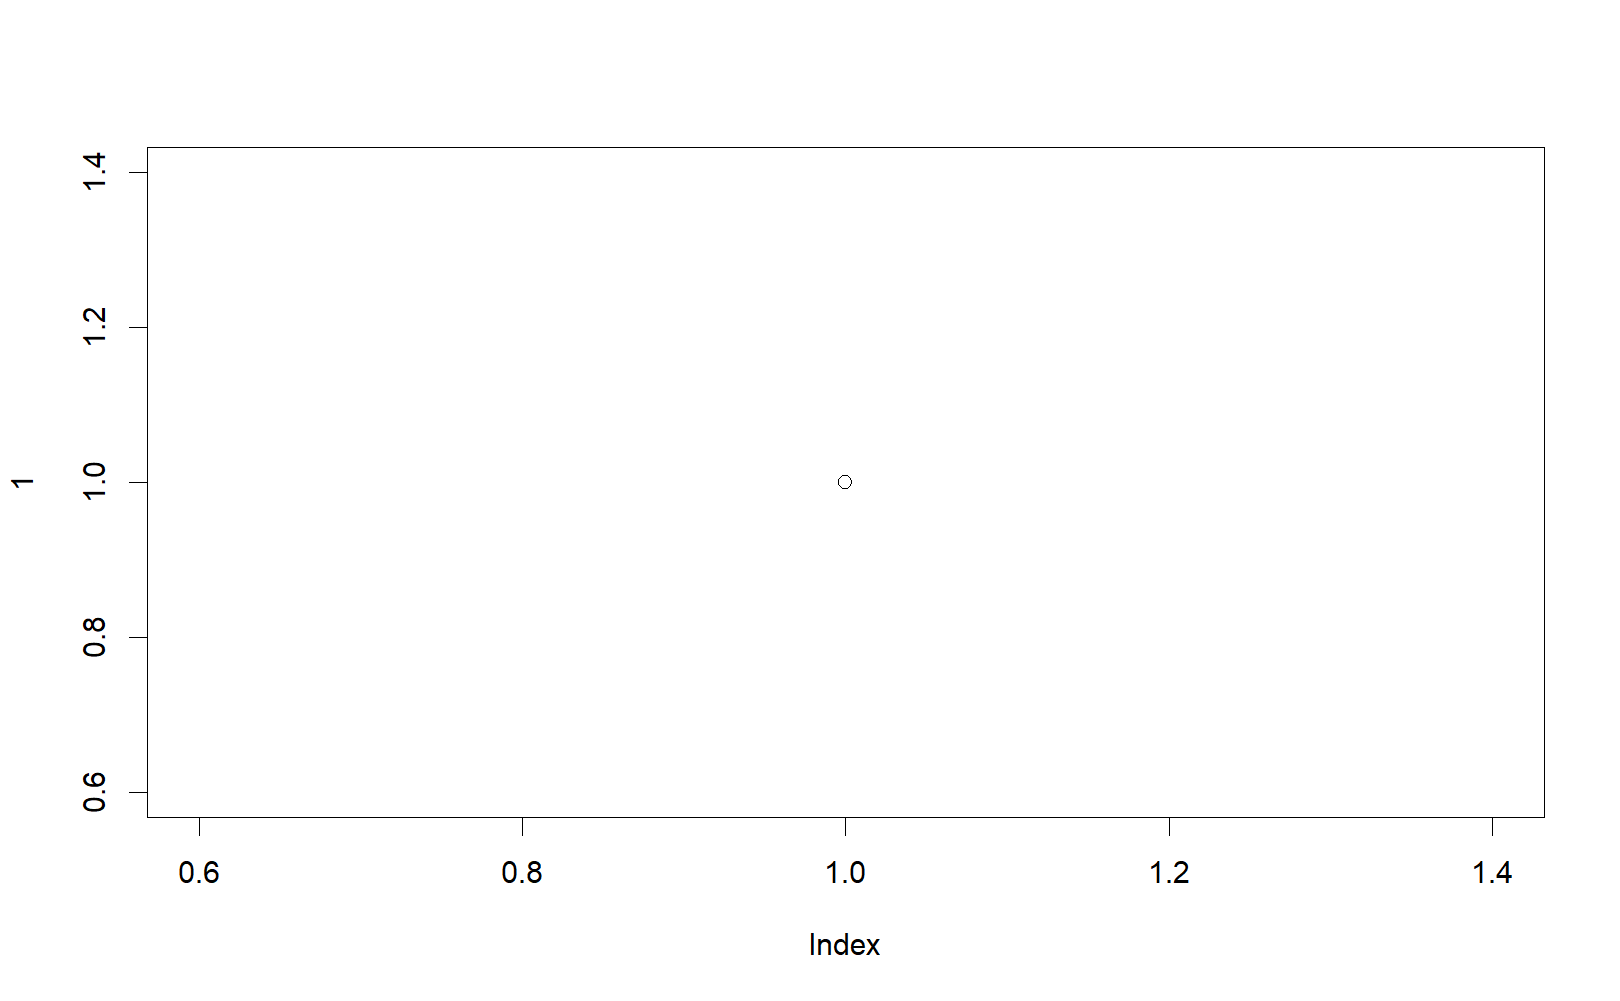
\includegraphics[width=6in]{knitr-figs-pdf/test1-1}}{Figure \ref{fig:test1}} 

}

\caption{Test}\label{fig:test1}
\end{figure}
\begin{longtable}[]{@{}lr@{}}
\caption{\label{tab:test2}Test}\tabularnewline
\toprule
x & y\tabularnewline
\midrule
\endfirsthead
\toprule
x & y\tabularnewline
\midrule
\endhead
a & 1\tabularnewline
a & 2\tabularnewline
b & 3\tabularnewline
\bottomrule
\end{longtable}
\begin{equation}
  1 + 1
  \label{eq:test2}
\end{equation}
See Figure~\ref{fig:test1} for the example appendix figure.

See Table~\ref{tab:test2} for the example appendix table.

\clearpage

\section{THE SECOND APPENDIX, FOR FUN}
\label{app:second-appendix}

More content.

\end{appendices}

\clearpage

\hypertarget{references}{%
\section{References}\label{references}}

\hypertarget{refs}{}
\leavevmode\hypertarget{ref-edwards2013}{}%
Edwards, A.M., Haigh, R., and Starr, P.J. 2014. Pacific Ocean Perch (\emph{Sebastes alutus}) stock assessment for the north and west coasts of Haida Gwaii, British Columbia. DFO Can. Sci. Advis. Sec. Res. Doc. 2013/092: vi + 126 p.
\end{document}
